\documentclass[10pt]{article}

\usepackage[a4paper,margin=0.72in]{geometry}
\usepackage[T1]{fontenc}
\usepackage[utf8]{inputenc}
\usepackage{array}
\usepackage{booktabs}
\usepackage{enumitem}
\usepackage{graphicx}
\usepackage{hyperref}
\usepackage{microtype}
\usepackage{pgfplots}
\usepackage{tabularx}
\usepackage{xcolor}

\pgfplotsset{compat=1.18}
\setlength{\parindent}{0pt}
\setlength{\parskip}{0.28em}
\setlength{\tabcolsep}{4pt}
\setlist[itemize]{leftmargin=*, itemsep=0.15em, topsep=0.15em}
\renewcommand{\arraystretch}{1.10}

\begin{document}

\begin{center}
  {\Large \textbf{Assignment 1: GPU-Accelerated Data Analysis}}\\[0.25em]
  Engineering of Data Analysis (2779)\\
  NOVA SBE\\[0.45em]
  \textbf{Project title:} \emph{GPU Acceleration of Complaint Dispute Classification}\\
  \textbf{Student(s):} [Connor Brown \& Vanessa Weiss]\\
  \textbf{Date:} 22 April 2026
\end{center}

{\small
\textbf{Submission note:} This report follows the assignment structure in \texttt{proj1.pdf}: pages 1--3 cover the performance analysis and page 4 documents AI-tool usage.
}

\section*{1. Problem Description}
This project predicts whether a consumer disputed a complaint using a structured-feature XGBoost classification pipeline built from the CFPB complaints dataset. The reduced assignment workflow keeps the predictive core of the original project while removing exploratory analysis, hyperparameter search, and interpretability sections so that the CPU baseline and GPU version can be compared cleanly.

The saved notebook outputs show a full cleaned training set of \textbf{321,430 rows}, an external inference set of \textbf{100 rows}, a full validation set of \textbf{64,286 rows}, and an encoded feature space of \textbf{3,375 columns}. These dimensions are large enough for model fitting to be computationally meaningful, especially once the one-hot encoded matrix is passed to XGBoost.

The CPU baseline uses pandas, NumPy, and XGBoost on CPU. The GPU solution keeps the same predictive task, features, splits, and model settings, but moves the dataframe and execution path to RAPIDS/cuDF, CuPy, and GPU-backed XGBoost. GPU acceleration is expected to help most in model training, where the workload is large and repeated across the dataset-size sweep.

\section*{2. Solution Design}
The porting strategy was intentionally conservative. Both notebooks use the same target, the same reduced structured feature set, the same deterministic subset fractions, the same random seed, the same classification threshold of 0.50, and the same XGBoost hyperparameters, with the only intentional model-level difference being \texttt{device='cpu'} versus \texttt{device='cuda'}.

The saved artifact summaries show that the two implementations remain structurally aligned at full scale: both produce 321,430 cleaned training rows, 100 inference rows, 3,375 encoded features, 64,286 validation predictions, and 100 inference predictions. The predictive metrics are also very close. At full scale, CPU and GPU F1 are 0.3851 and 0.3842 respectively, and the maximum absolute metric delta across the full sweep stays small (accuracy 0.0047, precision 0.0054, recall 0.0117, F1 0.0074). This supports the claim that the GPU notebook is a substantively equivalent implementation of the CPU baseline.

The saved CPU outputs were produced locally in a Windows VS Code Jupyter kernel, while the saved GPU outputs were produced in a WSL2 RAPIDS environment using an NVIDIA GeForce RTX 5080 Laptop GPU. The exact hardware and software stack used for both runs is documented in Section 7.

\section*{3. Experimental Setup}
The benchmark uses the assignment-style dataset-size sweep of 10\%, 25\%, 50\%, 75\%, and 100\% of the full cleaned dataset. Each benchmark point is repeated three times and the notebooks report mean and standard deviation. Three measured phases are reported: model training, validation inference on the held-out validation split, and external inference on the separate 100-row inference file.

Fairness controls are consistent across CPU and GPU. The notebooks use the same subset fractions, the same deterministic split logic, the same threshold, and the same evaluation metrics. GPU timing explicitly synchronizes before and after timed calls. One important scope detail is that the timed benchmark covers model execution only; preprocessing, split construction, and feature encoding are outside the timed blocks.

\begin{table}[h]
  \centering
  \footnotesize
  \begin{tabularx}{\linewidth}{>{\raggedright\arraybackslash}p{0.12\linewidth} >{\raggedleft\arraybackslash}p{0.15\linewidth} >{\raggedleft\arraybackslash}p{0.15\linewidth} >{\raggedleft\arraybackslash}p{0.12\linewidth} X}
    \toprule
    Dataset size & CPU total (s) & GPU total (s) & Speedup & Notes \\
    \midrule
    10\% & 7.8822 & 3.5634 & 2.21x & GPU already faster overall, but the tiny external inference batch still favors CPU. \\
    25\% & 16.7083 & 5.1354 & 3.25x & Training gains dominate the total measured improvement. \\
    50\% & 31.5068 & 8.2307 & 3.83x & Mid-scale run shows strong training acceleration with nearly identical F1. \\
    75\% & 47.2795 & 11.6053 & 4.07x & Best combined speedup in the saved results. \\
    100\% & 70.7750 & 18.5536 & 3.81x & Large full-scale GPU advantage persists. \\
    \bottomrule
  \end{tabularx}
  \caption{Combined measured workload time, where total time = training + validation inference + external inference.}
\end{table}

{\small
\textbf{Measured-scope note:} these timings do not include full raw-CSV-to-output preprocessing. They measure the model execution phases only.
}

\newpage

\section*{4. Results}
The saved notebook outputs show a clear overall GPU advantage. At full scale, the combined measured workload falls from \textbf{70.7750s} on CPU to \textbf{18.5536s} on GPU, which is a \textbf{3.81x} speedup. The GPU is already faster overall at 10\% scale, and the combined speedup grows to just above 4x at 75\% before settling at 3.81x for the full dataset.

\begin{center}
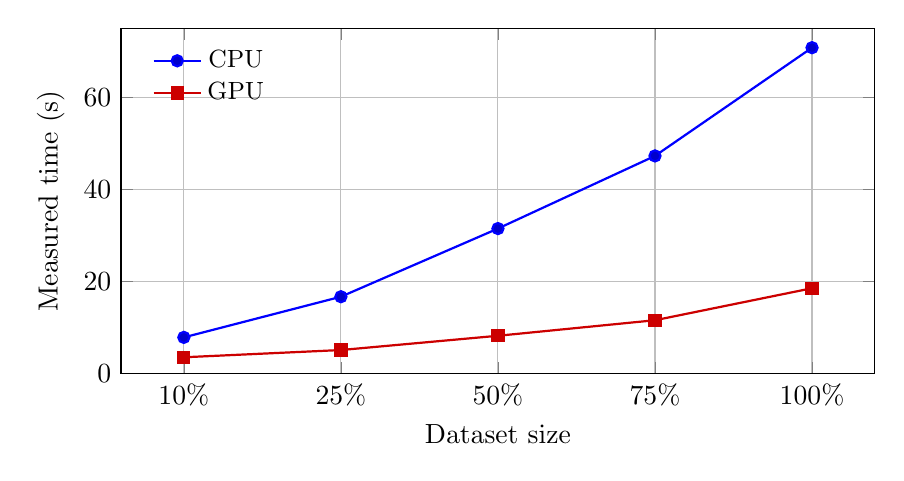
\begin{tikzpicture}
\begin{axis}[
    width=0.92\linewidth,
    height=2.35in,
    xlabel={Dataset size},
    ylabel={Measured time (s)},
    symbolic x coords={10,25,50,75,100},
    xtick=data,
    xticklabels={10\%,25\%,50\%,75\%,100\%},
    ymin=0,
    ymax=75,
    grid=major,
    legend style={draw=none, fill=none, font=\small, at={(0.03,0.97)}, anchor=north west}
]
\addplot+[mark=*, blue, thick] coordinates {
    (10,7.8822) (25,16.7083) (50,31.5068) (75,47.2795) (100,70.7750)
};
\addplot+[mark=square*, red!80!black, thick] coordinates {
    (10,3.5634) (25,5.1354) (50,8.2307) (75,11.6053) (100,18.5536)
};
\legend{CPU,GPU}
\end{axis}
\end{tikzpicture}
\end{center}

{\small
\textbf{Figure 1.} Combined measured workload time across the dataset-size sweep. The GPU series stays below the CPU series at every scale because the training phase dominates the measured workload.
}

\section*{5. Training vs. Inference Breakdown}
The gains are not uniform across phases. Training speedup ranges from \textbf{2.36x} to \textbf{4.24x}, with an average of about \textbf{3.61x}. Validation inference also benefits overall, with speedups from \textbf{1.02x} to \textbf{3.05x} and an average of about \textbf{1.78x}. In contrast, the external inference phase is slower on GPU at every scale because it only predicts 10--100 rows, which is too small to amortize GPU overhead.

Training is also the dominant share of measured time in both notebooks: \textbf{95.7\%--97.9\%} of CPU total measured time and \textbf{89.8\%--93.9\%} of GPU total measured time. That is why training acceleration translates so directly into overall speedup.

\begin{table}[h]
  \centering
  \small
  \begin{tabular}{lccc}
    \toprule
    Phase (100\% dataset) & CPU time (s) & GPU time (s) & Speedup \\
    \midrule
    Training & 69.2820 & 17.3749 & 3.99x \\
    Validation inference & 1.2309 & 0.7288 & 1.69x \\
    External inference & 0.2621 & 0.4499 & 0.58x \\
    \bottomrule
  \end{tabular}
  \caption{Full-scale phase-level timing breakdown.}
\end{table}

\newpage

\section*{6. Discussion}
The measured results support a clear but qualified conclusion. The GPU version is decisively better for model training, and because training dominates the measured workload, that benefit is strong enough to deliver a 2.21x--4.07x overall speedup across the sweep. This is the main practical result of the project.

The asymmetry between training and inference is also important. Validation inference benefits overall because the held-out validation set is still large enough to amortize some GPU setup overhead. External inference does not. The separate inference file contains only 100 rows at full scale, so the GPU pays kernel launch, synchronization, and memory-management overhead on a workload that is too small to benefit from parallel acceleration. This is consistent with the assignment requirement to discuss overheads such as memory movement, allocation, launch latency, and small-batch inefficiency.

One limitation is that the benchmark is not a full end-to-end pipeline benchmark. The notebooks time \texttt{fit} and \texttt{predict\_proba}, but not full preprocessing or encoding from raw CSV. Another limitation is visible in the CPU notebook output itself: repeated pandas fragmentation warnings appear during benchmark execution because the CPU column-alignment step inserts columns repeatedly. That probably adds some avoidable overhead to the baseline, although it does not change the main conclusion because the GPU training advantage is large and persistent.

Overall, the GPU benefit is strong enough to justify the extra complexity for repeated model training on medium-to-large subsets. It is much less compelling for tiny-batch inference.

\section*{7. Reproducibility Notes}
The submission includes the notebooks \path{complaints_assignment_cpu.ipynb} and \path{complaints_assignment_gpu.ipynb}, together with \path{complaints_training.csv} and \path{complaints_inference.csv}. The saved notebook outputs are sufficient to reproduce the comparison values reported here.

The CPU results were generated locally in the VS Code Jupyter front-end using the \path{C:\Users\conno\dev\envs\ml_lab\python.exe} environment on Windows 11 Home 64-bit (build 10.0.26200) with an Intel Core Ultra 9 275HX, 24 cores / 24 logical processors, 33.75 GB physical RAM, Python 3.13.12, and XGBoost 3.2.0. RAPIDS libraries were not installed in that CPU environment.

The GPU results were generated in a WSL2 RAPIDS environment on Ubuntu 24.04.4 LTS with an NVIDIA GeForce RTX 5080 Laptop GPU (16303 MiB VRAM), Python 3.13.13, XGBoost 3.2.0, cuDF 26.04.00, CuPy 14.0.1, cuML 26.04.00, and CUDA 13.1. The GPU notebook uses explicit synchronization for timing.

The same GPU notebook was also tested successfully in a Google Colab GPU runtime, confirming that the implementation runs in the course-required Colab environment even though the benchmark values reported here come from the WSL2 RAPIDS run.

\section*{8. Conclusion}
The GPU notebook is a substantively equivalent implementation of the CPU baseline and delivers meaningful performance gains for the measured workload. The strongest benefit appears in training, where GPU execution provides roughly 4x speedup at the larger scales. Validation inference also improves overall, but tiny external inference batches remain CPU-favored because GPU overhead is not amortized.

For this project, the GPU version is preferable when the workflow is training-heavy or repeatedly fits the model on medium-to-large datasets. The CPU version remains adequate for very small-batch inference and for environments where GPU setup complexity is not justified.

\newpage

\section*{9. AI Tools Usage}
This project used \textbf{OpenAI Codex} as the primary AI assistant inside an agent-style coding workflow. The tool was used to restructure the notebooks, align the CPU and GPU implementations, diagnose environment-specific runtime issues, extract saved benchmark outputs, and draft the report support files. The model used in this workflow was a \textbf{GPT-5.4-based Codex agent}. If the course requires a more precise platform-side model label, that should be copied from the IDE or account logs before submission.

\subsection*{9.1 Tools and Models Used}
\begin{itemize}
  \item \textbf{Tool:} OpenAI Codex
  \item \textbf{Model:} GPT-5.4-based Codex agent
  \item \textbf{Scope:} notebook simplification, CPU/GPU alignment, WSL/RAPIDS runtime debugging, benchmark extraction, analysis drafting, and report drafting
\end{itemize}

\subsection*{9.2 Interaction Mode}
\begin{itemize}
  \item The workflow was primarily \textbf{agentic}: the assistant inspected files, proposed plans, edited notebooks and report files, and carried out multi-step refactors.
  \item It also included a conversational component: the student used short follow-up prompts to redirect work, refine scope, and approve plan changes before implementation.
\end{itemize}

\subsection*{9.3 Development Strategy}
\begin{itemize}
  \item \textbf{Closest strategy used:} Benchmark-guided
  \item \textbf{Why:} performance data from the saved CPU and GPU notebook outputs drove the later stages of the work, especially when deciding what to analyze in the report and how to interpret the CPU vs GPU differences by phase.
  \item There was also a design-first element earlier in the process when the notebooks were restructured to keep the CPU and GPU pipelines comparable before analyzing performance.
\end{itemize}

\subsection*{9.4 Reflection}
\begin{itemize}
  \item \textbf{What worked well:} the AI assistant was effective at repetitive notebook cleanup, keeping the CPU and GPU logic aligned, extracting benchmark outputs into structured tables, and turning those outputs into report-ready narrative.
  \item \textbf{What did not work well:} environment-dependent GPU issues still required careful manual interpretation, especially when moving between the local Windows CPU kernel and the WSL2 RAPIDS GPU environment. The assistant could help with notebook structure and debugging, but environment mismatches still needed human intervention and management.
  \item \textbf{Influence on the final solution:} AI use accelerated implementation and reporting, but the final conclusions still depend on human validation of the measured outputs, environment assumptions, and the benchmark scope.
\end{itemize}


\end{document}
